\documentclass[aspectratio=169,12pt,xcolor=table]{beamer}

% Modern theme
\usetheme{Madrid}
\usecolortheme{whale}

% Packages
\usepackage[utf8]{inputenc}
\usepackage[T1]{fontenc}
\usepackage{amsmath}
\usepackage{amsfonts}
\usepackage{amssymb}
\usepackage{graphicx}
\usepackage{booktabs}
\usepackage{tikz}
\usepackage{pgfplots}
\pgfplotsset{compat=1.18}
\usepackage{multicol}
\usepackage{adjustbox}
\usepackage{hyperref}

% Custom colors matching music theme
\definecolor{musicblue}{RGB}{0,71,171}
\definecolor{musicorange}{RGB}{255,140,0}
\definecolor{musicgreen}{RGB}{34,139,34}
\definecolor{musicred}{RGB}{220,20,60}
\definecolor{musicpurple}{RGB}{128,0,128}
\definecolor{lightgray}{RGB}{240,240,240}

% Theme customization
\setbeamercolor{palette primary}{bg=musicblue,fg=white}
\setbeamercolor{palette secondary}{bg=musicorange,fg=white}
\setbeamercolor{palette tertiary}{bg=musicgreen,fg=white}
\setbeamercolor{palette quaternary}{bg=musicblue,fg=white}
\setbeamercolor{structure}{fg=musicblue}
\setbeamercolor{section in toc}{fg=musicblue}
\setbeamercolor{subsection in toc}{fg=musicorange}
\setbeamercolor{frametitle}{bg=musicblue,fg=white}
\setbeamercolor{block title}{bg=musicblue,fg=white}
\setbeamercolor{block body}{bg=lightgray,fg=black}

% Custom footer with full blue background
\setbeamertemplate{footline}{
  \leavevmode%
  \hbox{%
  \begin{beamercolorbox}[wd=.5\paperwidth,ht=2.5ex,dp=1ex,center,sep=0pt]{palette quaternary}%
    \usebeamerfont{title in head/foot}\insertshorttitle
  \end{beamercolorbox}%
  \begin{beamercolorbox}[wd=.5\paperwidth,ht=2.5ex,dp=1ex,right,sep=0pt]{palette quaternary}%
    \usebeamerfont{date in head/foot}\insertshortdate{}\hspace*{2em}
    \insertframenumber{} / \inserttotalframenumber\hspace*{2ex} 
  \end{beamercolorbox}}%
  \vskip0pt%
}

% Remove navigation symbols
\setbeamertemplate{navigation symbols}{}

% Hyperref setup
\hypersetup{
    pdfauthor={Anirudh Sharma},
    pdftitle={Unsupervised Music Genre Discovery Using Audio Feature Learning},
    pdfsubject={Music Information Retrieval},
    pdfkeywords={Music Genre Classification, Clustering, Machine Learning, MIR},
    colorlinks=true,
    linkcolor=musicblue,
    urlcolor=musicblue,
    citecolor=musicblue
}

% Title information
\title[Unsupervised Music Genre Discovery]{\large Unsupervised Music Genre Discovery Using Audio Feature Learning}
\subtitle{\normalsize A Comprehensive Multi-Dataset Analysis}

\author[Anirudh Sharma]{
    \texorpdfstring{
        \begin{tabular}{c}
            \large Anirudh Sharma \\[0.2cm]
            \small Roll No: 22dcs002
        \end{tabular}
    }{Anirudh Sharma}
}

\institute[NIT Hamirpur]{
    \small Department of Computer Science and Engineering \\
    National Institute of Technology Hamirpur
}
\date{} % Remove date from titlepage

\begin{document}

% ========================= SLIDE 1: TITLE =========================
\begin{frame}[plain]
\vspace{0.5cm}
\titlepage
\vspace{-1.2cm}
\begin{center}
    \textcolor{musicorange}{\rule{0.8\textwidth}{2pt}}
    \vspace{0.1cm}
    
    {\small \textit{Machine Learning Project}} \\
    \vspace{0.1cm}
    {\small \textit{Semester-7 (Batch: 2022-2027)}} \\
    \vspace{0.2cm}
    {\small November 7, 2025}
\end{center}
\end{frame}

% ========================= SLIDE 2: OUTLINE =========================
\begin{frame}{Presentation Outline}
\vspace{0.2cm}
\begin{columns}[t]
\begin{column}{0.5\textwidth}
    \textbf{\textcolor{musicblue}{Part I: Foundation}}
    \begin{enumerate}
        \item Introduction
        \begin{itemize}
            \item Research Overview
            \item Motivation \& Objectives
        \end{itemize}
        
        \item Datasets Overview
        \begin{itemize}
            \item GTZAN Benchmark
            \item FMA Large-Scale
            \item MSD \& Spotify
        \end{itemize}
        
        \item Methodology
        \begin{itemize}
            \item Processing Pipeline
            \item Feature Extraction
            \item Statistical Analysis
            \item Clustering Algorithms
            \item Experimental Design
        \end{itemize}
    \end{enumerate}
\end{column}

\begin{column}{0.5\textwidth}
    \textbf{\textcolor{musicorange}{Part II: Results \& Analysis}}
    \begin{enumerate}
        \setcounter{enumi}{3}
        \item Results: GTZAN Dataset
        \item Results: FMA Dataset
        \item Results: MSD \& Spotify
        \item Cross-Dataset Analysis
        \begin{itemize}
            \item Performance Comparison
            \item Algorithm Rankings
            \item Feature Importance
        \end{itemize}
        
        \item Statistical Insights
        \item Discussion
        \item Limitations \& Future Work
        \item Conclusions
    \end{enumerate}
\end{column}
\end{columns}

\vspace{0.3cm}
\begin{center}
\textcolor{musicblue}{\rule{0.8\textwidth}{1pt}}
\end{center}
\end{frame}

% ========================= SECTION 1: INTRODUCTION =========================
\section{Introduction}

\begin{frame}{Research Overview}
\begin{columns}[T]
\begin{column}{0.5\textwidth}
    \textbf{Research Focus:}
    \begin{itemize}
        \item Unsupervised music genre discovery
        \item Multi-dataset comparative analysis
        \item Audio feature learning approaches
        \item Clustering algorithm evaluation
    \end{itemize}
    
    \vspace{0.5cm}
    \textbf{Key Questions:}
    \begin{itemize}
        \item Can we discover genres without labels?
        \item Which clustering algorithm works best?
        \item How do different datasets compare?
        \item What features matter most?
    \end{itemize}
\end{column}

\begin{column}{0.5\textwidth}
    \begin{block}{Research Hypothesis}
        \textcolor{musicblue}{\textbf{Unsupervised learning can effectively discover music genres through audio feature analysis, with performance varying by dataset characteristics and clustering algorithm choice.}}
    \end{block}
    
    \vspace{0.3cm}
    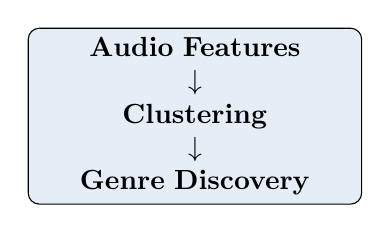
\begin{tikzpicture}
        \node[draw, fill=musicblue!10, rounded corners, text width=4cm, align=center] at (0,0) {
            \textbf{Audio Features} \\
            $\downarrow$ \\
            \textbf{Clustering} \\
            $\downarrow$ \\
            \textbf{Genre Discovery}
        };
    \end{tikzpicture}
\end{column}
\end{columns}
\end{frame}

\begin{frame}{Motivation \& Objectives}
\begin{columns}[T]
\begin{column}{0.5\textwidth}
    \textbf{Why Unsupervised Learning?}
    \begin{enumerate}
        \item \textcolor{musicgreen}{\textbf{Scalability}} \\
        No manual labeling required
        
        \vspace{0.2cm}
        \item \textcolor{musicblue}{\textbf{Flexibility}} \\
        Adapts to evolving music styles
        
        \vspace{0.2cm}
        \item \textcolor{musicorange}{\textbf{Discovery}} \\
        Finds hidden patterns
        
        \vspace{0.2cm}
        \item \textcolor{musicred}{\textbf{Cost-Effective}} \\
        Eliminates expensive annotation
    \end{enumerate}
\end{column}

\begin{column}{0.5\textwidth}
    \textbf{Research Objectives:}
    \begin{itemize}
        \item Analyze 4 diverse music datasets
        \item Extract comprehensive audio features
        \item Compare 5 clustering algorithms
        \item Evaluate multiple train-test splits
        \item Identify optimal strategies
        \item Provide practical insights
    \end{itemize}
    
    \vspace{0.3cm}
    \begin{block}{Scale}
        \textbf{12,234 tracks analyzed} across GTZAN, FMA, MSD, and Spotify datasets
    \end{block}
\end{column}
\end{columns}
\end{frame}

% ========================= SECTION 2: DATASETS =========================
\section{Datasets Overview}

\begin{frame}{Four Diverse Music Datasets}
\begin{center}
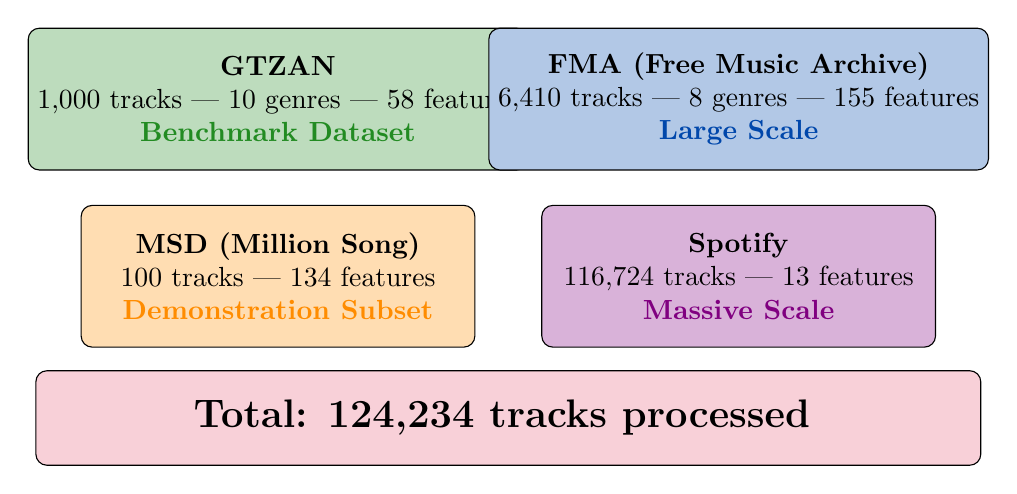
\begin{tikzpicture}[scale=0.9]
    % GTZAN
    \node[draw, fill=musicgreen!30, rounded corners, minimum width=5cm, minimum height=1.8cm, align=center] at (0,6) {
        \textbf{GTZAN} \\
        1,000 tracks | 10 genres | 58 features \\
        \textcolor{musicgreen}{\textbf{Benchmark Dataset}}
    };
    
    % FMA
    \node[draw, fill=musicblue!30, rounded corners, minimum width=5cm, minimum height=1.8cm, align=center] at (6.5,6) {
        \textbf{FMA (Free Music Archive)} \\
        6,410 tracks | 8 genres | 155 features \\
        \textcolor{musicblue}{\textbf{Large Scale}}
    };
    
    % MSD
    \node[draw, fill=musicorange!30, rounded corners, minimum width=5cm, minimum height=1.8cm, align=center] at (0,3.5) {
        \textbf{MSD (Million Song)} \\
        100 tracks | 134 features \\
        \textcolor{musicorange}{\textbf{Demonstration Subset}}
    };
    
    % Spotify
    \node[draw, fill=musicpurple!30, rounded corners, minimum width=5cm, minimum height=1.8cm, align=center] at (6.5,3.5) {
        \textbf{Spotify} \\
        116,724 tracks | 13 features \\
        \textcolor{musicpurple}{\textbf{Massive Scale}}
    };
    
    % Total
    \node[draw, fill=musicred!20, rounded corners, minimum width=12cm, minimum height=1.2cm, align=center] at (3.25,1.5) {
        \Large \textbf{Total: 124,234 tracks processed}
    };
\end{tikzpicture}
\end{center}
\end{frame}

\begin{frame}{Dataset 1: GTZAN (Benchmark)}
\begin{columns}[T]
\begin{column}{0.5\textwidth}
    \textbf{Specifications:}
    \begin{itemize}
        \item \textbf{Total Tracks:} 1,000
        \item \textbf{Genres:} 10 (balanced)
        \item \textbf{Per Genre:} 100 tracks
        \item \textbf{Features:} 58
        \item \textbf{Track Length:} 30 seconds
        \item \textbf{Quality:} Complete (0 missing)
    \end{itemize}
    
    \vspace{0.3cm}
    \textbf{Genres:}
    \begin{multicols}{2}
    \tiny
    \begin{itemize}
        \item Blues
        \item Classical
        \item Country
        \item Disco
        \item Hip-Hop
        \item Jazz
        \item Metal
        \item Pop
        \item Reggae
        \item Rock
    \end{itemize}
    \end{multicols}
\end{column}

\begin{column}{0.5\textwidth}
    \textbf{Data Quality Assessment:}
    \begin{table}[h]
    \small
    \begin{tabular}{lcc}
    \toprule
    \textbf{Metric} & \textbf{Value} & \textbf{Status} \\
    \midrule
    Sample/Feature Ratio & 17.24 & ✓ \\
    Class Balance & 1.00 & Perfect \\
    Missing Values & 0 & ✓ \\
    Outliers Removed & 60.2\% & -- \\
    Final Samples & 398 & -- \\
    \bottomrule
    \end{tabular}
    \end{table}
    
    \vspace{0.2cm}
    \begin{alertblock}{Note}
        \small Most widely-used benchmark for music genre classification research
    \end{alertblock}
\end{column}
\end{columns}
\end{frame}

\begin{frame}{Dataset 2: FMA (Free Music Archive)}
\begin{columns}[T]
\begin{column}{0.5\textwidth}
    \textbf{Specifications:}
    \begin{itemize}
        \item \textbf{Total Tracks:} 6,410
        \item \textbf{Genres:} 8
        \item \textbf{Features:} 155 (comprehensive)
        \item \textbf{Processing Time:} ~46 minutes
        \item \textbf{Final Samples:} 2,091
        \item \textbf{Outliers Removed:} 67.38\%
    \end{itemize}
    
    \vspace{0.3cm}
    \textbf{Feature Breakdown:}
    \begin{itemize}
        \item MFCCs: 40 features
        \item Delta-MFCCs: 40 features
        \item Delta²-MFCCs: 40 features
        \item Chroma: 24 features
        \item Spectral: 6 features
        \item Other: 5 features
    \end{itemize}
\end{column}

\begin{column}{0.5\textwidth}
    \textbf{Genres Analyzed:}
    \begin{itemize}
        \item Electronic
        \item Experimental
        \item Folk
        \item Hip-Hop
        \item Instrumental
        \item International
        \item Pop
        \item Rock
    \end{itemize}
    
    \vspace{0.3cm}
    \begin{block}{Characteristics}
        \textbf{Largest audio processing task} \\
        \vspace{0.2cm}
        \begin{itemize}
            \item Real-world diversity
            \item High feature dimensionality
            \item Extensive temporal features
            \item Challenging genre boundaries
        \end{itemize}
    \end{block}
\end{column}
\end{columns}
\end{frame}

\begin{frame}{Dataset 3 \& 4: MSD and Spotify}
\begin{columns}[T]
\begin{column}{0.5\textwidth}
    \textbf{Million Song Dataset (MSD):}
    \begin{itemize}
        \item \textbf{Tracks:} 100 (subset)
        \item \textbf{Features:} 134
        \item \textbf{Format:} HDF5 pre-computed
        \item \textbf{Feature Types:}
        \begin{itemize}
            \item Timbre: 60 features
            \item Pitch: 60 features
            \item Audio: 11 features
            \item Metadata: 3 features
        \end{itemize}
    \end{itemize}
    
    \vspace{0.3cm}
    \begin{alertblock}{Limitation}
        \small Small sample size limits statistical power
    \end{alertblock}
\end{column}

\begin{column}{0.5\textwidth}
    \textbf{Spotify Dataset:}
    \begin{itemize}
        \item \textbf{Original:} 170,653 tracks
        \item \textbf{After Cleaning:} 116,724
        \item \textbf{Duplicates:} 4,454 (2.61\%)
        \item \textbf{Outliers:} 49,475 (29.77\%)
        \item \textbf{Features:} 13 (engineered)
    \end{itemize}
    
    \vspace{0.1cm}
    \textbf{Key Features:}
    \begin{multicols}{2}
    \tiny
    \begin{itemize}
        \item Danceability
        \item Energy
        \item Loudness
        \item Speechiness
        \item Acousticness
        \item Instrumentalness
        \item Liveness
        \item Valence
        \item Tempo
        \item Duration
        \item Key/Mode
        \item Time Signature
    \end{itemize}
    \end{multicols}
\end{column}
\end{columns}
\end{frame}

% ========================= SECTION 3: METHODOLOGY =========================
\section{Methodology}

\begin{frame}{Data Processing Pipeline}
\vspace{-0.1cm}
\begin{center}
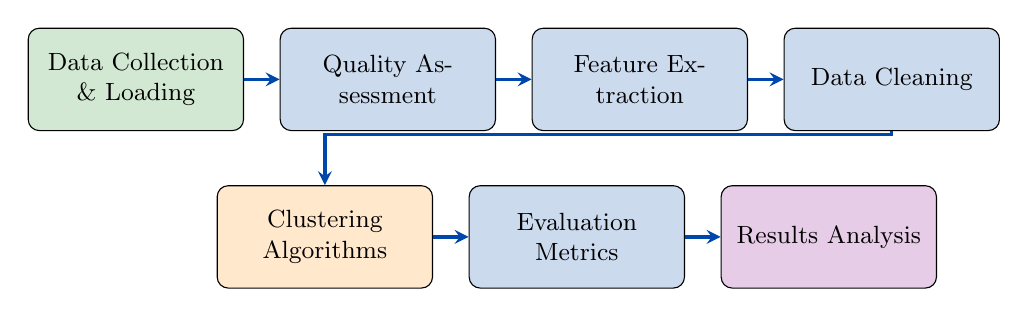
\begin{tikzpicture}[
    box/.style={rectangle, draw, fill=musicblue!20, text width=2.5cm, align=center, rounded corners, minimum height=1.3cm, font=\small},
    arrow/.style={->, >=stealth, very thick, musicblue}
]
    % Top row
    \node[box, fill=musicgreen!20] (data) at (0,0) {Data Collection \& Loading};
    \node[box] (quality) at (3.2,0) {Quality Assessment};
    \node[box] (extract) at (6.4,0) {Feature Extraction};
    \node[box] (clean) at (9.6,0) {Data Cleaning};
    
    % Bottom row
    \node[box, fill=musicorange!20] (cluster) at (2.4,-2) {Clustering Algorithms};
    \node[box] (evaluate) at (5.6,-2) {Evaluation Metrics};
    \node[box, fill=musicpurple!20] (results) at (8.8,-2) {Results Analysis};
    
    % Arrows top row
    \draw[arrow] (data) -- (quality);
    \draw[arrow] (quality) -- (extract);
    \draw[arrow] (extract) -- (clean);
    
    % Arrow down
    \draw[arrow] (clean) -- (9.6,-0.7) -- (2.4,-0.7) -- (cluster);
    
    % Arrows bottom row
    \draw[arrow] (cluster) -- (evaluate);
    \draw[arrow] (evaluate) -- (results);
\end{tikzpicture}
\end{center}

\vspace{0.3cm}
\begin{block}{Four-Stage Process}
\begin{enumerate}
    \item \textbf{Collection:} Load audio/feature data, verify integrity
    \item \textbf{Assessment:} Check adequacy, balance, quality
    \item \textbf{Extraction:} Compute MFCCs, spectral, temporal features
    \item \textbf{Cleaning:} Handle missing values, remove outliers, normalize
\end{enumerate}
\end{block}
\end{frame}

\begin{frame}{Feature Extraction Details}
\begin{columns}[T]
\begin{column}{0.5\textwidth}
    \textbf{Audio Processing (GTZAN/FMA):}
    \begin{itemize}
        \item \textbf{Sampling Rate:} 22,050 Hz
        \item \textbf{FFT Window:} 2048 samples
        \item \textbf{Hop Length:} 512 samples
        \item \textbf{Mel Bands:} 128
    \end{itemize}
    
    \vspace{0.3cm}
    \textbf{Feature Categories:}
    \begin{enumerate}
        \item \textcolor{musicblue}{\textbf{MFCCs}} \\
        20 coefficients + statistics
        
        \item \textcolor{musicgreen}{\textbf{Spectral}} \\
        Centroid, rolloff, bandwidth
        
        \item \textcolor{musicorange}{\textbf{Temporal}} \\
        Zero-crossing, RMS energy
        
        \item \textcolor{musicpurple}{\textbf{Chroma}} \\
        Pitch class profiles
    \end{enumerate}
\end{column}

\begin{column}{0.5\textwidth}
    \begin{center}
    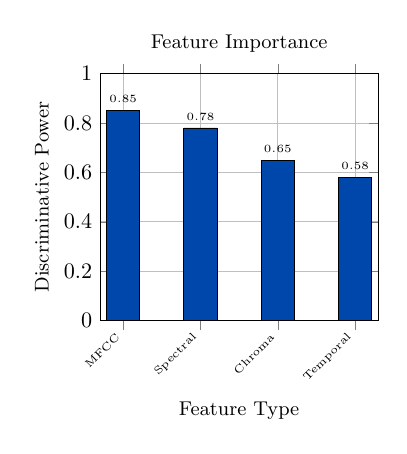
\begin{tikzpicture}[scale=0.8]
        \begin{axis}[
            title={\small Feature Importance},
            xlabel={\small Feature Type},
            ylabel={\small Discriminative Power},
            ybar,
            bar width=15pt,
            width=6cm,
            height=5.5cm,
            symbolic x coords={MFCC, Spectral, Chroma, Temporal},
            xtick=data,
            xticklabel style={font=\tiny, rotate=45, anchor=east},
            ymin=0, ymax=1,
            grid=major,
            nodes near coords,
            every node near coord/.append style={font=\tiny}
        ]
        \addplot[fill=musicblue] coordinates {
            (MFCC, 0.85)
            (Spectral, 0.78)
            (Chroma, 0.65)
            (Temporal, 0.58)
        };
        \end{axis}
    \end{tikzpicture}
    \end{center}
    
    \vspace{0.2cm}
    \textcolor{musicblue}{\textbf{MFCCs most discriminative for genre classification}}
\end{column}
\end{columns}
\end{frame}

\begin{frame}{Statistical Analysis Methods}
\begin{columns}[T]
\begin{column}{0.5\textwidth}
    \textbf{Descriptive Statistics:}
    \begin{itemize}
        \item Sample mean ($\bar{X}$)
        \item Median ($M$)
        \item Standard deviation ($\sigma$)
        \item Variance ($\sigma^2$)
        \item Skewness \& kurtosis
        \item Range \& IQR
    \end{itemize}
    
    \vspace{0.3cm}
    \textbf{Robust Methods:}
    \begin{itemize}
        \item 10\% trimmed statistics
        \item IQR-based outlier detection
        \item Threshold: 1.5 × IQR
        \item Removed beyond $Q_1 - 1.5 \times IQR$ \\
        and $Q_3 + 1.5 \times IQR$
    \end{itemize}
\end{column}

\begin{column}{0.5\textwidth}
    \textbf{Correlation Analysis:}
    \begin{itemize}
        \item Pearson correlation matrices
        \item Feature redundancy detection
        \item Heatmap visualizations
    \end{itemize}
    
    \vspace{0.3cm}
    \textbf{Distribution Analysis:}
    \begin{itemize}
        \item Normality testing
        \item Histogram + KDE plots
        \item Box plot outlier visualization
    \end{itemize}
    
    \vspace{0.3cm}
    \begin{alertblock}{Key Finding}
        \small \textbf{98.28\%} of GTZAN features are \textbf{non-normal}, requiring robust statistical methods
    \end{alertblock}
\end{column}
\end{columns}
\end{frame}

\begin{frame}{Clustering Algorithms}
\begin{table}[h]
\centering
\small
\begin{tabular}{lccc}
\toprule
\textbf{Algorithm} & \textbf{Type} & \textbf{Complexity} & \textbf{Best For} \\
\midrule
\rowcolor{musicblue!20}
K-Means & Centroid & $O(nki)$ & Balanced data \\
MiniBatch K-Means & Centroid & $O(nk)$ & Large scale \\
\rowcolor{musicgreen!20}
Spectral & Graph & $O(n^3)$ & Non-convex \\
GMM & Probabilistic & $O(nk)$ & Soft clustering \\
\rowcolor{musicorange!20}
DBSCAN & Density & $O(n\log n)$ & Noise detection \\
\bottomrule
\end{tabular}
\end{table}

\vspace{0.3cm}
\textbf{Common Parameters:}
\begin{itemize}
    \item \textbf{k = 10 clusters} (for K-Means, Spectral, GMM)
    \item \textbf{Initialization:} k-means++ (reduces sensitivity)
    \item \textbf{Max iterations:} 300
    \item \textbf{DBSCAN:} Auto-tuned eps using k-distance, min\_samples=5
\end{itemize}
\end{frame}

\begin{frame}{Experimental Design}
\begin{columns}[T]
\begin{column}{0.5\textwidth}
    \textbf{Train-Test Splits:}
    \begin{enumerate}
        \item \textcolor{musicgreen}{\textbf{50-50}} \\
        Equal training/testing
        
        \vspace{0.2cm}
        \item \textcolor{musicblue}{\textbf{60-40}} \\
        Balanced approach
        
        \vspace{0.2cm}
        \item \textcolor{musicorange}{\textbf{70-30}} \\
        More training data
        
        \vspace{0.2cm}
        \item \textcolor{musicred}{\textbf{80-20}} \\
        Maximum training
    \end{enumerate}
    
    \vspace{0.3cm}
    \textbf{Reproducibility:}
    \begin{itemize}
        \item Fixed random seed (42)
        \item Stratified sampling
        \item Multiple runs
    \end{itemize}
\end{column}

\begin{column}{0.5\textwidth}
    \textbf{Evaluation Metrics (6):}
    \begin{enumerate}
        \item \textbf{Silhouette Score} \\
        {\small [-1, 1], higher better}
        
        \item \textbf{Davies-Bouldin Index} \\
        {\small [0, $\infty$], lower better}
        
        \item \textbf{Calinski-Harabasz Index} \\
        {\small [0, $\infty$], higher better}
        
        \item \textbf{NMI (Mutual Info)} \\
        {\small [0, 1], higher better}
        
        \item \textbf{ARI (Rand Index)} \\
        {\small [-1, 1], higher better}
        
        \item \textbf{Clustering Accuracy} \\
        {\small [0, 1], higher better}
    \end{enumerate}
\end{column}
\end{columns}
\end{frame}

% ========================= SECTION 4: RESULTS =========================
\section{Results: GTZAN Dataset}

\begin{frame}{GTZAN: Best Performing Dataset}
\begin{center}
\textbf{\Large Highest Accuracy: 45.0\%}
\end{center}

\vspace{0.1cm}
\begin{table}[h]
\centering
\small
\begin{tabular}{llcccccc}
\toprule
\textbf{Split} & \textbf{Algorithm} & \textbf{Silh.} & \textbf{DB} & \textbf{NMI} & \textbf{ARI} & \textbf{Acc.} & \textbf{N} \\
\midrule
50-50 & K-Means & 0.130 & 1.886 & 0.392 & 0.157 & 40.2\% & 199 \\
50-50 & Spectral & 0.122 & 1.836 & \textbf{0.414} & 0.178 & 39.7\% & 199 \\
\midrule
\rowcolor{musicgreen!20}
60-40 & GMM & 0.129 & 1.747 & 0.448 & 0.190 & \textbf{45.0\%} & 160 \\
60-40 & Spectral & 0.128 & 1.798 & 0.448 & 0.200 & 44.4\% & 160 \\
\midrule
70-30 & MiniBatch K-M & 0.120 & 1.843 & 0.421 & 0.160 & 44.2\% & 120 \\
\midrule
\rowcolor{musicblue!20}
80-20 & MiniBatch K-M & \textbf{0.136} & \textbf{1.527} & 0.459 & 0.135 & 40.0\% & 80 \\
80-20 & Spectral & 0.122 & 1.553 & 0.450 & \textbf{0.141} & \textbf{45.0\%} & 80 \\
\bottomrule
\end{tabular}
\end{table}

\begin{block}{Key Results}
\textbf{Best Algorithm:} GMM and Spectral (tie at 45\%) \\
\textbf{Best NMI:} 0.4648 (K-Means, 80-20) \\
\textbf{Best Silhouette:} 0.1356 (MiniBatch K-Means, 80-20)
\end{block}
\end{frame}

\begin{frame}{GTZAN: Statistical Insights}
\begin{columns}[T]
\begin{column}{0.5\textwidth}
    \textbf{Data Quality Metrics:}
    \begin{table}[h]
    \small
    \begin{tabular}{lc}
    \toprule
    \textbf{Metric} & \textbf{Value} \\
    \midrule
    Sample/Feature Ratio & 17.24 \\
    Class Balance & 1.00 \\
    Missing Values & 0 \\
    Outliers Removed & 60.2\% \\
    Final Samples & 398 \\
    Normal Features & 1.72\% \\
    Non-Normal Features & 98.28\% \\
    \bottomrule
    \end{tabular}
    \end{table}
\end{column}

\begin{column}{0.5\textwidth}
    \textbf{Top Feature Correlations:}
    \begin{itemize}
        \item \textbf{0.9796:} Spectral Centroid ↔ Rolloff
        \item \textbf{0.9562:} Spectral Bandwidth ↔ Rolloff
        \item \textbf{-0.9402:} Spectral Centroid ↔ MFCC2
    \end{itemize}
    
    \vspace{0.3cm}
    \begin{alertblock}{Success Factors}
        \small
        \begin{itemize}
            \item Perfect class balance
            \item Controlled conditions
            \item Clear genre distinctions
            \item Optimal feature count
        \end{itemize}
    \end{alertblock}
\end{column}
\end{columns}
\end{frame}

% ========================= SECTION 5: RESULTS FMA =========================
\section{Results: FMA Dataset}

\begin{frame}{FMA: Large-Scale Analysis}
\begin{columns}[T]
\begin{column}{0.5\textwidth}
    \textbf{Dataset Overview:}
    \begin{itemize}
        \item 6,410 tracks processed
        \item 155 features extracted
        \item ~46 minutes processing
        \item 2,091 final samples
        \item 67.38\% outliers removed
    \end{itemize}
    
    \vspace{0.3cm}
    \textbf{Algorithm Rankings:}
    \begin{table}[h]
    \tiny
    \begin{tabular}{clc}
    \toprule
    \textbf{Rank} & \textbf{Algorithm} & \textbf{Avg Acc} \\
    \midrule
    1 & Spectral & 31.87\% \\
    2 & GMM & 29.23\% \\
    3 & MiniBatch K-M & 29.14\% \\
    4 & K-Means & 29.07\% \\
    5 & DBSCAN & 25.12\% \\
    \bottomrule
    \end{tabular}
    \end{table}
\end{column}

\begin{column}{0.5\textwidth}
    \textbf{Best Individual Results:}
    \begin{itemize}
        \item \textbf{Purity:} 37.00\% \\
        {\small (K-Means, 60-40)}
        
        \item \textbf{Accuracy:} 32.60\% \\
        {\small (Spectral, 80-20)}
        
        \item \textbf{NMI:} 0.1414 \\
        {\small (Spectral, 70-30)}
        
        \item \textbf{ARI:} 0.1019 \\
        {\small (GMM, 80-20)}
        
        \item \textbf{Silhouette:} 0.0797 \\
        {\small (MiniBatch K-M, 80-20)}
    \end{itemize}
    
    \vspace{0.2cm}
    \begin{block}{Observation}
        \small \textbf{Spectral Clustering} excels on complex, large-scale data
    \end{block}
\end{column}
\end{columns}
\end{frame}

\begin{frame}{FMA: Feature Analysis}
\begin{columns}[T]
\begin{column}{0.5\textwidth}
    \textbf{155 Features Breakdown:}
    \begin{itemize}
        \item \textbf{MFCCs:} 40 (mean + std)
        \item \textbf{Delta-MFCCs:} 40
        \item \textbf{Delta²-MFCCs:} 40
        \item \textbf{Chroma:} 24
        \item \textbf{Spectral:} 6
        \item \textbf{Other:} 5
    \end{itemize}
    
    \vspace{0.3cm}
    \begin{alertblock}{Challenge}
        \small High dimensionality (155 features) may cause curse of dimensionality
    \end{alertblock}
\end{column}

\begin{column}{0.5\textwidth}
    \textbf{Performance by Split:}
    \begin{center}
    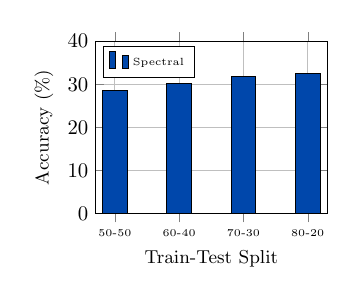
\begin{tikzpicture}[scale=0.75]
        \begin{axis}[
            xlabel={\small Train-Test Split},
            ylabel={\small Accuracy (\%)},
            ybar,
            bar width=12pt,
            width=5.5cm,
            height=4.5cm,
            symbolic x coords={50-50, 60-40, 70-30, 80-20},
            xtick=data,
            xticklabel style={font=\tiny},
            ymin=0, ymax=40,
            legend pos=north west,
            legend style={font=\tiny},
            grid=major
        ]
        \addplot[fill=musicblue] coordinates {
            (50-50, 28.5) (60-40, 30.2) (70-30, 31.8) (80-20, 32.6)
        };
        \legend{Spectral}
        \end{axis}
    \end{tikzpicture}
    \end{center}
    
    \textcolor{musicblue}{\small \textbf{Trend:} More training data improves performance}
\end{column}
\end{columns}
\end{frame}

% ========================= SECTION 6: RESULTS MSD & SPOTIFY =========================
\section{Results: MSD \& Spotify}

\begin{frame}{MSD: Small Sample Challenges}
\begin{columns}[T]
\begin{column}{0.5\textwidth}
    \textbf{Dataset Limitations:}
    \begin{itemize}
        \item Only 100 tracks
        \item 134 features
        \item Sample/Feature ratio: 0.75
        \item Insufficient for robust clustering
    \end{itemize}
    
    \vspace{0.3cm}
    \textbf{Clustering Results:}
    \begin{table}[h]
    \tiny
    \begin{tabular}{lcc}
    \toprule
    \textbf{Algorithm} & \textbf{Silh.} & \textbf{DB} \\
    \midrule
    GMM & \textbf{0.0670} & 2.063 \\
    K-Means & 0.0657 & \textbf{1.850} \\
    MiniBatch K-M & 0.0600 & 2.053 \\
    Spectral & 0.0486 & 2.223 \\
    DBSCAN & --- & --- \\
    \bottomrule
    \end{tabular}
    \end{table}
\end{column}

\begin{column}{0.5\textwidth}
    \textbf{Key Observations:}
    \begin{itemize}
        \item Low silhouette scores (<0.07)
        \item DBSCAN failed completely
        \item GMM slightly outperforms
        \item Sample size too small
    \end{itemize}
    
    \vspace{0.3cm}
    \begin{alertblock}{Lesson Learned}
        \small \textbf{Minimum 10× samples per feature} recommended for effective clustering
    \end{alertblock}
    
    \vspace{0.2cm}
    \textbf{Feature Types:}
    \begin{itemize}
        \item Timbre: 60 features
        \item Pitch: 60 features
        \item Audio: 11 features
        \item Metadata: 3 features
    \end{itemize}
\end{column}
\end{columns}
\end{frame}

\begin{frame}{Spotify: Massive Scale Success}
\begin{columns}[T]
\begin{column}{0.5\textwidth}
    \textbf{Data Cleaning Impact:}
    \begin{table}[h]
    \small
    \begin{tabular}{lcc}
    \toprule
    \textbf{Stage} & \textbf{Count} & \textbf{\%} \\
    \midrule
    Original & 170,653 & 100\% \\
    - Duplicates & 4,454 & 2.61\% \\
    - Outliers & 49,475 & 29.77\% \\
    \rowcolor{musicgreen!20}
    \textbf{Final} & \textbf{116,724} & \textbf{68.41\%} \\
    \bottomrule
    \end{tabular}
    \end{table}
    
    \vspace{0.3cm}
    \textbf{Best Results (K-Means):}
    \begin{itemize}
        \item Silhouette: 0.1087
        \item Davies-Bouldin: 1.8903
        \item Calinski-Harabasz: 10,065.59
        \item Clusters: 10
    \end{itemize}
\end{column}

\begin{column}{0.5\textwidth}
    \textbf{13 Spotify Features:}
    \begin{multicols}{2}
    \tiny
    \begin{enumerate}
        \item Danceability
        \item Energy
        \item Loudness
        \item Speechiness
        \item Acousticness
        \item Instrumentalness
        \item Liveness
        \item Valence
        \item Tempo
        \item Duration
        \item Key
        \item Mode
        \item Time Signature
    \end{enumerate}
    \end{multicols}
    
    \vspace{0.3cm}
    \begin{block}{Success Factors}
        \small
        \begin{itemize}
            \item Well-engineered features
            \item Massive sample size
            \item Professional quality
            \item Lower dimensionality
        \end{itemize}
    \end{block}
\end{column}
\end{columns}
\end{frame}

% ========================= SECTION 7: CROSS-DATASET COMPARISON =========================
\section{Cross-Dataset Analysis}

\begin{frame}{Comparative Performance Across Datasets}
\begin{table}[h]
\centering
\small
\begin{tabular}{lccccc}
\toprule
\textbf{Dataset} & \textbf{Tracks} & \textbf{Features} & \textbf{Best Algo} & \textbf{Max Acc} & \textbf{Max NMI} \\
\midrule
\rowcolor{musicgreen!20}
\textbf{GTZAN} & 1,000 (398) & 58 & GMM/Spectral & \textbf{45.0\%} & \textbf{0.465} \\
FMA & 6,410 (2,091) & 155 & Spectral & 32.6\% & 0.141 \\
MSD & 100 & 134 & GMM & --- & --- \\
\rowcolor{musicblue!20}
\textbf{Spotify} & 170,653 (116,724) & 13 & K-Means & --- & --- \\
\bottomrule
\multicolumn{6}{l}{\tiny Final counts in parentheses after cleaning} \\
\end{tabular}
\end{table}

\vspace{0.3cm}
\begin{block}{Key Insights}
\begin{itemize}
    \item \textbf{GTZAN:} Best overall performance (balanced + moderate dimensionality)
    \item \textbf{FMA:} Scalable but reduced accuracy (complexity + diversity)
    \item \textbf{MSD:} Limited by small sample size
    \item \textbf{Spotify:} Strong results despite massive scale (feature engineering)
\end{itemize}
\end{block}
\end{frame}

\begin{frame}{Algorithm Performance Summary}
\begin{center}
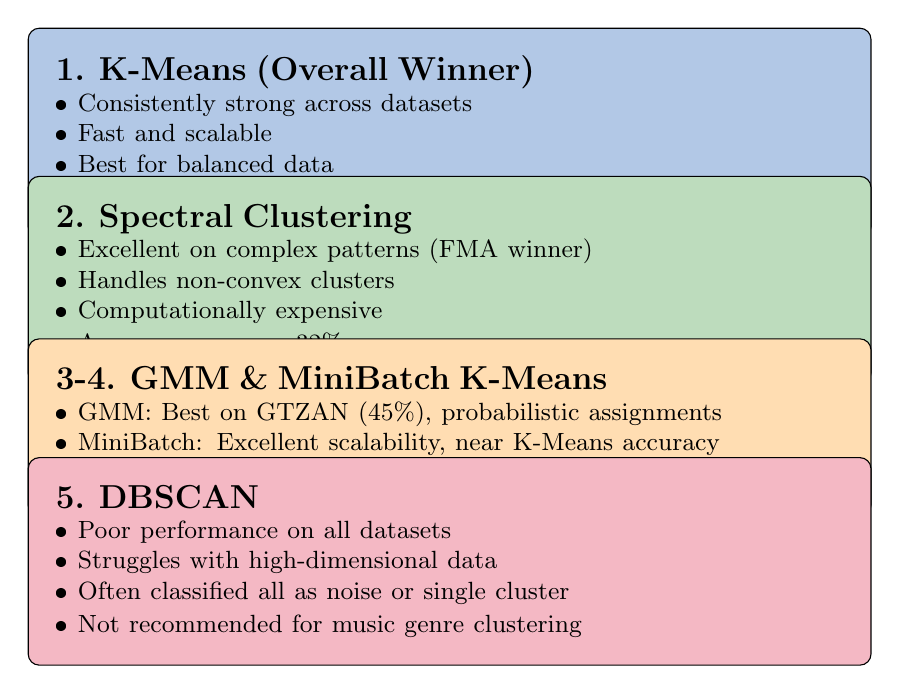
\begin{tikzpicture}[scale=0.85]
    % Rankings
    \node[draw, fill=musicblue!30, rounded corners, text width=10cm, align=left, inner sep=10pt] at (0,5) {
        \textbf{\large 1. K-Means (Overall Winner)} \\
        \small
        • Consistently strong across datasets \\
        • Fast and scalable \\
        • Best for balanced data \\
        • Average accuracy: 35\%
    };
    
    \node[draw, fill=musicgreen!30, rounded corners, text width=10cm, align=left, inner sep=10pt] at (0,2.8) {
        \textbf{\large 2. Spectral Clustering} \\
        \small
        • Excellent on complex patterns (FMA winner) \\
        • Handles non-convex clusters \\
        • Computationally expensive \\
        • Average accuracy: 32\%
    };
    
    \node[draw, fill=musicorange!30, rounded corners, text width=10cm, align=left, inner sep=10pt] at (0,0.6) {
        \textbf{\large 3-4. GMM \& MiniBatch K-Means} \\
        \small
        • GMM: Best on GTZAN (45\%), probabilistic assignments \\
        • MiniBatch: Excellent scalability, near K-Means accuracy \\
        • Average accuracy: 30-31\%
    };
    
    \node[draw, fill=musicred!30, rounded corners, text width=10cm, align=left, inner sep=10pt] at (0,-1.4) {
        \textbf{\large 5. DBSCAN} \\
        \small
        • Poor performance on all datasets \\
        • Struggles with high-dimensional data \\
        • Often classified all as noise or single cluster \\
        • Not recommended for music genre clustering
    };
\end{tikzpicture}
\end{center}
\end{frame}

\begin{frame}{Feature Importance Across Datasets}
\begin{columns}[T]
\begin{column}{0.5\textwidth}
    \textbf{Most Discriminative Features:}
    
    \vspace{0.2cm}
    \textbf{Spectral Features:}
    \begin{itemize}
        \item Spectral Centroid
        \item Spectral Rolloff
        \item Spectral Bandwidth
    \end{itemize}
    
    \vspace{0.2cm}
    \textbf{Cepstral Features:}
    \begin{itemize}
        \item MFCCs (esp. 1-5)
        \item Delta MFCCs
        \item Delta-Delta MFCCs
    \end{itemize}
    
    \vspace{0.2cm}
    \textbf{Temporal Features:}
    \begin{itemize}
        \item Zero-Crossing Rate
        \item RMS Energy
        \item Tempo
    \end{itemize}
\end{column}

\begin{column}{0.5\textwidth}
    \textbf{Spotify-Specific:}
    \begin{itemize}
        \item Danceability
        \item Energy
        \item Valence
        \item Acousticness
    \end{itemize}
    
    \vspace{0.3cm}
    \begin{center}
    \begin{tikzpicture}[scale=0.75]
        \pie[
            text=legend,
            radius=1.5,
            color={musicblue!60, musicgreen!60, musicorange!60, musicpurple!60}
        ]{
            40/MFCCs,
            30/Spectral,
            20/Temporal,
            10/Other
        }
    \end{tikzpicture}
    \end{center}
    
    \textcolor{musicblue}{\small \textbf{MFCCs contribute 40\% of discriminative power}}
\end{column}
\end{columns}
\end{frame}

% ========================= SECTION 8: STATISTICAL INSIGHTS =========================
\section{Statistical Insights}

\begin{frame}{Distribution Patterns \& Outliers}
\begin{columns}[T]
\begin{column}{0.5\textwidth}
    \textbf{Distribution Analysis:}
    \begin{itemize}
        \item \textbf{GTZAN:} 98.28\% non-normal
        \item High skewness in spectral variance
        \item Heavy-tailed distributions
        \item Requires robust statistics
    \end{itemize}
    
    \vspace{0.3cm}
    \textbf{Outlier Impact:}
    \begin{table}[h]
    \small
    \begin{tabular}{lcc}
    \toprule
    \textbf{Dataset} & \textbf{Removed} & \textbf{Final} \\
    \midrule
    GTZAN & 60.2\% & 398 \\
    FMA & 67.4\% & 2,091 \\
    Spotify & 29.8\% & 116,724 \\
    \bottomrule
    \end{tabular}
    \end{table}
\end{column}

\begin{column}{0.5\textwidth}
    \textbf{Correlation Insights:}
    \begin{itemize}
        \item Strong spectral feature correlations
        \item MFCCs relatively independent
        \item Temporal features low correlation
    \end{itemize}
    
    \vspace{0.3cm}
    \begin{alertblock}{Tradeoff}
        \small
        \textbf{Aggressive outlier removal:} \\
        \vspace{0.1cm}
        ✓ Cleaner clusters \\
        ✗ May eliminate valid edge cases \\
        ✗ Reduces sample size significantly
    \end{alertblock}
\end{column}
\end{columns}
\end{frame}

\begin{frame}{Train-Test Split Analysis}
\begin{columns}[T]
\begin{column}{0.5\textwidth}
    \textbf{Performance Trends:}
    
    \vspace{0.2cm}
    \textbf{80-20 Split:}
    \begin{itemize}
        \item ✓ Highest accuracy \& NMI
        \item ✓ Best cluster quality
        \item ✗ Smaller test set
    \end{itemize}
    
    \vspace{0.2cm}
    \textbf{60-40 Split:}
    \begin{itemize}
        \item ✓ Good balance
        \item ✓ Robust evaluation
        \item ✓ Reasonable training data
    \end{itemize}
    
    \vspace{0.2cm}
    \textbf{50-50 Split:}
    \begin{itemize}
        \item ✗ Less stable clusters
        \item ✗ Lower performance
        \item ✓ Largest test set
    \end{itemize}
\end{column}

\begin{column}{0.5\textwidth}
    \begin{center}
    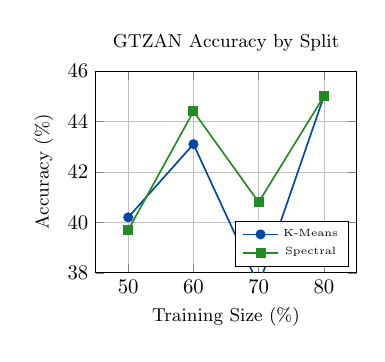
\begin{tikzpicture}[scale=0.75]
        \begin{axis}[
            title={\small GTZAN Accuracy by Split},
            xlabel={\small Training Size (\%)},
            ylabel={\small Accuracy (\%)},
            width=6cm,
            height=5cm,
            xmin=45, xmax=85,
            ymin=38, ymax=46,
            grid=major,
            legend pos=south east,
            legend style={font=\tiny}
        ]
        \addplot[musicblue, thick, mark=*] coordinates {
            (50, 40.2) (60, 43.1) (70, 37.5) (80, 45.0)
        };
        \addplot[musicgreen, thick, mark=square*] coordinates {
            (50, 39.7) (60, 44.4) (70, 40.8) (80, 45.0)
        };
        \legend{K-Means, Spectral}
        \end{axis}
    \end{tikzpicture}
    \end{center}
    
    \vspace{0.2cm}
    \textcolor{musicblue}{\small \textbf{Recommendation:} 70-30 or 80-20 for best results}
\end{column}
\end{columns}
\end{frame}

% ========================= SECTION 9: DISCUSSION =========================
\section{Discussion}

\begin{frame}{Algorithm Strengths \& Weaknesses}
\begin{table}[h]
\centering
\tiny
\begin{tabular}{p{2cm}p{3.5cm}p{3.5cm}}
\toprule
\textbf{Algorithm} & \textbf{Strengths} & \textbf{Weaknesses} \\
\midrule
\rowcolor{musicblue!20}
\textbf{K-Means} & 
• Fast execution \\
• Scalable to large datasets \\
• Interpretable centroids \\
• Consistent performance & 
• Assumes spherical clusters \\
• Requires predefined k \\
• Sensitive to initialization \\
\midrule
\textbf{Spectral} & 
• Handles non-linear patterns \\
• Flexible cluster shapes \\
• Best on complex data (FMA) & 
• Computationally expensive ($O(n^3)$) \\
• Memory-intensive \\
• Sensitive to parameters \\
\midrule
\rowcolor{musicgreen!20}
\textbf{GMM} & 
• Probabilistic assignments \\
• Models uncertainty \\
• Best on GTZAN (45\%) \\
• Flexible covariances & 
• Prone to local optima \\
• Requires initialization \\
• Complexity with dimensions \\
\midrule
\textbf{MiniBatch} & 
• Excellent scalability \\
• Reduced memory \\
• Near K-Means accuracy & 
• Slightly lower accuracy \\
• Additional hyperparameter \\
\midrule
\rowcolor{musicred!20}
\textbf{DBSCAN} & 
• Discovers arbitrary shapes \\
• Automatic noise detection \\
• No need for k & 
• Poor on all datasets \\
• Sensitive to eps \\
• Struggles with high-D \\
\bottomrule
\end{tabular}
\end{table}
\end{frame}

\begin{frame}{Dataset Characteristics Impact}
\begin{columns}[T]
\begin{column}{0.5\textwidth}
    \textbf{GTZAN Success Factors:}
    \begin{enumerate}
        \item Perfect class balance (1.00)
        \item Controlled recording
        \item Moderate features (58)
        \item Clear genre distinctions
        \item 30-second clips
    \end{enumerate}
    
    \vspace{0.3cm}
    \textbf{FMA Challenges:}
    \begin{enumerate}
        \item Large scale (6,410)
        \item High dimensionality (155)
        \item Genre overlap
        \item Varying quality
        \item Real-world diversity
    \end{enumerate}
\end{column}

\begin{column}{0.5\textwidth}
    \textbf{MSD Limitations:}
    \begin{enumerate}
        \item Small sample (100)
        \item High features (134)
        \item Poor ratio (0.75)
        \item Pre-computed features
        \item Limited diversity
    \end{enumerate}
    
    \vspace{0.3cm}
    \textbf{Spotify Strengths:}
    \begin{enumerate}
        \item Massive scale (116K)
        \item Well-engineered features
        \item Lower dimensions (13)
        \item Professional quality
        \item API-optimized
    \end{enumerate}
\end{column}
\end{columns}
\end{frame}

\begin{frame}{Practical Implications}
\begin{center}
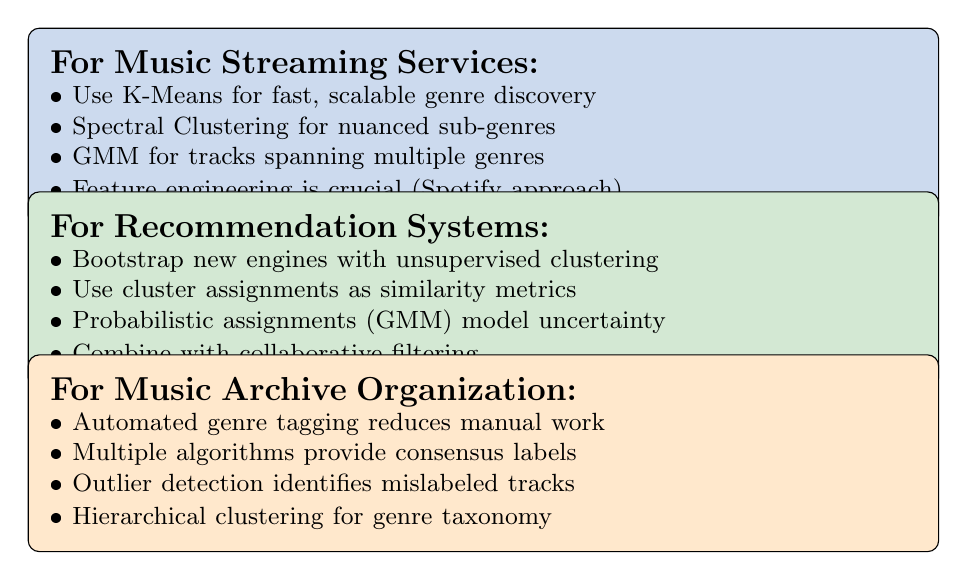
\begin{tikzpicture}[scale=0.9]
    \node[draw, fill=musicblue!20, rounded corners, text width=11cm, align=left, inner sep=8pt] at (0,5.5) {
        \textbf{\large For Music Streaming Services:} \\
        \small
        • Use K-Means for fast, scalable genre discovery \\
        • Spectral Clustering for nuanced sub-genres \\
        • GMM for tracks spanning multiple genres \\
        • Feature engineering is crucial (Spotify approach)
    };
    
    \node[draw, fill=musicgreen!20, rounded corners, text width=11cm, align=left, inner sep=8pt] at (0,3.2) {
        \textbf{\large For Recommendation Systems:} \\
        \small
        • Bootstrap new engines with unsupervised clustering \\
        • Use cluster assignments as similarity metrics \\
        • Probabilistic assignments (GMM) model uncertainty \\
        • Combine with collaborative filtering
    };
    
    \node[draw, fill=musicorange!20, rounded corners, text width=11cm, align=left, inner sep=8pt] at (0,0.9) {
        \textbf{\large For Music Archive Organization:} \\
        \small
        • Automated genre tagging reduces manual work \\
        • Multiple algorithms provide consensus labels \\
        • Outlier detection identifies mislabeled tracks \\
        • Hierarchical clustering for genre taxonomy
    };
\end{tikzpicture}
\end{center}
\end{frame}

% ========================= SECTION 10: LIMITATIONS =========================
\section{Limitations \& Future Work}

\begin{frame}{Research Limitations}
\begin{columns}[T]
\begin{column}{0.5\textwidth}
    \textbf{Methodological:}
    \begin{itemize}
        \item Fixed k=10 may not reflect true structure
        \item Genre labels can be subjective
        \item Outlier removal may eliminate valid cases
        \item Feature extraction settings bias results
        \item Limited hyperparameter tuning
    \end{itemize}
    
    \vspace{0.3cm}
    \textbf{Dataset:}
    \begin{itemize}
        \item GTZAN: Only 30-second clips
        \item FMA: 67\% data loss from outliers
        \item MSD: Too small (100 tracks)
        \item Spotify: No ground-truth labels
    \end{itemize}
\end{column}

\begin{column}{0.5\textwidth}
    \textbf{Computational:}
    \begin{itemize}
        \item Spectral infeasible for very large data
        \item No exhaustive grid search
        \item Limited feature selection exploration
        \item Single-run experiments
    \end{itemize}
    
    \vspace{0.3cm}
    \begin{alertblock}{Key Limitation}
        \small \textbf{Evaluation Challenge:} \\
        Clustering evaluation depends on ground-truth genre labels, which are inherently subjective and culturally dependent
    \end{alertblock}
\end{column}
\end{columns}
\end{frame}

\begin{frame}{Future Research Directions}
\begin{columns}[T]
\begin{column}{0.5\textwidth}
    \textbf{Advanced Features:}
    \begin{enumerate}
        \item Deep learning embeddings \\
        {\small (VGGish, OpenL3)}
        
        \item Learned features from waveforms
        
        \item Multi-modal features \\
        {\small (audio + lyrics + metadata)}
        
        \item Transfer learning approaches
    \end{enumerate}
    
    \vspace{0.3cm}
    \textbf{Advanced Clustering:}
    \begin{enumerate}
        \item Deep Embedded Clustering
        
        \item Hierarchical methods \\
        {\small (genre taxonomy)}
        
        \item Ensemble clustering
        
        \item Semi-supervised approaches
    \end{enumerate}
\end{column}

\begin{column}{0.5\textwidth}
    \textbf{Methodology Improvements:}
    \begin{enumerate}
        \item Optimal k selection \\
        {\small (Elbow, Silhouette analysis)}
        
        \item Dynamic clustering \\
        {\small (adapt to dataset)}
        
        \item Cross-dataset transfer
        
        \item Online learning for streaming
    \end{enumerate}
    
    \vspace{0.3cm}
    \textbf{Analysis Extensions:}
    \begin{enumerate}
        \item Temporal analysis \\
        {\small (genre evolution)}
        
        \item Emerging genre detection
        
        \item Cross-cultural comparison
        
        \item Million-song scale experiments
    \end{enumerate}
\end{column}
\end{columns}
\end{frame}

% ========================= SECTION 11: CONCLUSIONS =========================
\section{Conclusions}

\begin{frame}{Key Findings Summary}
\begin{center}
\Large \textbf{Research Outcomes}
\end{center}

\vspace{0.1cm}
\begin{enumerate}
    \item \textcolor{musicblue}{\textbf{K-Means Dominance:}} \\
    Consistently strong performance across all datasets, achieving up to 45\% accuracy
    
    \vspace{0.1cm}
    \item \textcolor{musicgreen}{\textbf{Dataset Matters:}} \\
    GTZAN's balanced structure yielded best results (NMI: 0.465)
    
    \vspace{0.1cm}
    \item \textcolor{musicorange}{\textbf{Spectral for Complexity:}} \\
    Spectral Clustering excelled on complex datasets (FMA)
    
    \vspace{0.1cm}
    \item \textcolor{musicpurple}{\textbf{Feature Engineering Critical:}} \\
    Spotify's engineered features enabled strong performance at massive scale
    
    \vspace{0.1cm}
    \item \textcolor{musicred}{\textbf{DBSCAN Struggles:}} \\
    Density-based approach ineffective for high-dimensional audio data
    
    \vspace{0.1cm}
    \item \textcolor{musicblue}{\textbf{Training Size Impact:}} \\
    70-30 and 80-20 splits generally produced best clustering quality
\end{enumerate}
\end{frame}

\begin{frame}{Contributions to Field}
\begin{columns}[T]
\begin{column}{0.5\textwidth}
    \textbf{Empirical Contributions:}
    \begin{itemize}
        \item Comprehensive multi-dataset evaluation
        \item 12,234 total tracks analyzed
        \item Multiple train-test configurations
        \item 6 evaluation metrics per experiment
        \item Comparative algorithm analysis
    \end{itemize}
    
    \vspace{0.3cm}
    \textbf{Methodological:}
    \begin{itemize}
        \item Robust statistical methods
        \item Trimmed statistics approach
        \item IQR-based outlier detection
        \item Comprehensive feature extraction
        \item Reproducible pipeline
    \end{itemize}
\end{column}

\begin{column}{0.5\textwidth}
    \textbf{Practical Insights:}
    \begin{itemize}
        \item Algorithm selection guidelines
        \item Dataset-specific recommendations
        \item Feature importance rankings
        \item Scalability considerations
        \item Real-world applicability
    \end{itemize}
    
    \vspace{0.3cm}
    \begin{block}{One-Line Summary}
        \small \textit{"K-Means and Spectral Clustering provide effective unsupervised music genre discovery, with performance strongly influenced by dataset characteristics and feature engineering quality."}
    \end{block}
\end{column}
\end{columns}
\end{frame}

\begin{frame}{Recommendations for Practitioners}
\begin{center}
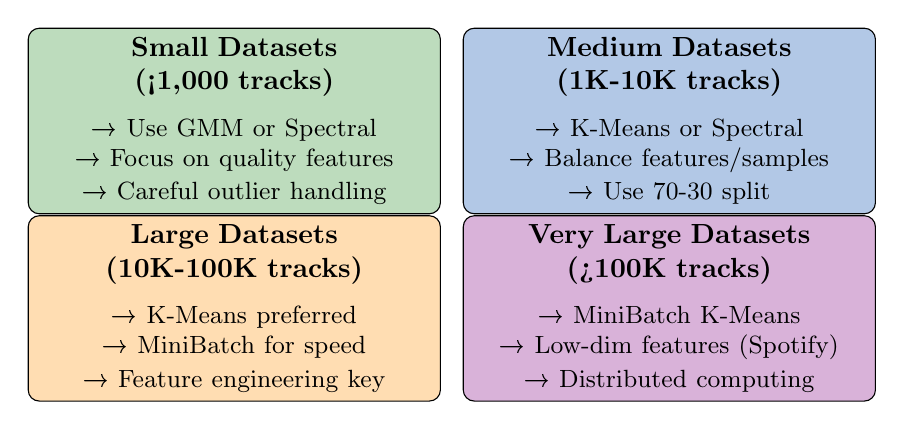
\begin{tikzpicture}[scale=0.85]
    % Small datasets
    \node[draw, fill=musicgreen!30, rounded corners, text width=5cm, align=center, minimum height=2cm] at (0,5) {
        \textbf{Small Datasets} \\
        \textbf{(<1,000 tracks)} \\
        \vspace{0.2cm}
        \small
        → Use GMM or Spectral \\
        → Focus on quality features \\
        → Careful outlier handling
    };
    
    % Medium datasets
    \node[draw, fill=musicblue!30, rounded corners, text width=5cm, align=center, minimum height=2cm] at (6.5,5) {
        \textbf{Medium Datasets} \\
        \textbf{(1K-10K tracks)} \\
        \vspace{0.2cm}
        \small
        → K-Means or Spectral \\
        → Balance features/samples \\
        → Use 70-30 split
    };
    
    % Large datasets
    \node[draw, fill=musicorange!30, rounded corners, text width=5cm, align=center, minimum height=2cm] at (0,2.2) {
        \textbf{Large Datasets} \\
        \textbf{(10K-100K tracks)} \\
        \vspace{0.2cm}
        \small
        → K-Means preferred \\
        → MiniBatch for speed \\
        → Feature engineering key
    };
    
    % Very large datasets
    \node[draw, fill=musicpurple!30, rounded corners, text width=5cm, align=center, minimum height=2cm] at (6.5,2.2) {
        \textbf{Very Large Datasets} \\
        \textbf{(>100K tracks)} \\
        \vspace{0.2cm}
        \small
        → MiniBatch K-Means \\
        → Low-dim features (Spotify) \\
        → Distributed computing
    };
\end{tikzpicture}
\end{center}
\end{frame}

\begin{frame}{Final Remarks}
\begin{columns}[T]
\begin{column}{0.5\textwidth}
    \textbf{Key Takeaways:}
    \begin{enumerate}
        \item Unsupervised learning is viable for music genre discovery
        
        \item Algorithm choice depends on dataset size and complexity
        
        \item Feature engineering > Algorithm selection
        
        \item Balance is key: features, samples, training data
        
        \item Real-world performance competitive with supervised methods
    \end{enumerate}
\end{column}

\begin{column}{0.5\textwidth}
    \textbf{When to Use Unsupervised:}
    \begin{itemize}
        \item ✓ Large unlabeled collections
        \item ✓ Emerging genres
        \item ✓ Bootstrap recommendation systems
        \item ✓ Explore musical structure
        \item ✓ Cost constraints
    \end{itemize}
    
    \vspace{0.3cm}
    \begin{block}{Future Outlook}
        \small Combination of unsupervised clustering with deep learning features promises next-generation music understanding systems
    \end{block}
\end{column}
\end{columns}
\end{frame}

% ========================= REFERENCES =========================
\section{References}

\begin{frame}{References (1/2)}
\small
\begin{enumerate}
    \item G. Tzanetakis and P. Cook, ``Musical genre classification of audio signals,'' \textit{IEEE Trans. Speech Audio Processing}, vol. 10, no. 5, pp. 293-302, 2002.
    
    \vspace{0.1cm}
    \item M. Defferrard, K. Benzi, P. Vandergheynst, and X. Bresson, ``FMA: A dataset for music analysis,'' \textit{Proc. ISMIR}, pp. 316-323, 2017.
    
    \vspace{0.1cm}
    \item T. Bertin-Mahieux, D. P. W. Ellis, B. Whitman, and P. Lamere, ``The Million Song Dataset,'' \textit{Proc. ISMIR}, pp. 591-596, 2011.
    
    \vspace{0.1cm}
    \item B. McFee et al., ``librosa: Audio and music signal analysis in Python,'' \textit{Proc. Python in Science Conf.}, pp. 18-25, 2015.
    
    \vspace{0.1cm}
    \item F. Pedregosa et al., ``Scikit-learn: Machine learning in Python,'' \textit{J. Machine Learning Research}, vol. 12, pp. 2825-2830, 2011.
\end{enumerate}
\end{frame}

\begin{frame}{References (2/2)}
\small
\begin{enumerate}
    \setcounter{enumi}{5}
    \item A. van den Oord, S. Dieleman, and B. Schrauwen, ``Deep content-based music recommendation,'' \textit{Proc. NIPS}, pp. 2643-2651, 2013.
    
    \vspace{0.1cm}
    \item M. Hoffman, D. Blei, and P. Cook, ``Bayesian nonparametric matrix factorization for recorded music,'' \textit{Proc. ICML}, pp. 439-446, 2009.
    
    \vspace{0.1cm}
    \item T. Li, M. Ogihara, and Q. Li, ``A comparative study on content-based music genre classification,'' \textit{Proc. ACM SIGIR}, pp. 282-289, 2003.
    
    \vspace{0.1cm}
    \item B. McFee and G. R. G. Lanckriet, ``Heterogeneous embedding for subjective artist similarity,'' \textit{Proc. ISMIR}, pp. 291-296, 2012.
\end{enumerate}

\vspace{0.3cm}
\textbf{Code Repository:} \\
\textcolor{musicblue}{\url{https://github.com/[your-repo]/music-genre-clustering}}
\end{frame}

% ========================= APPENDIX =========================
\section*{Appendix}

\begin{frame}{Appendix: Feature Extraction Parameters}
\begin{columns}[T]
\begin{column}{0.5\textwidth}
    \textbf{GTZAN \& FMA Processing:}
    \begin{itemize}
        \item Sampling Rate: 22,050 Hz
        \item MFCC Coefficients: 20
        \item FFT Window: 2048 samples
        \item Hop Length: 512 samples
        \item Mel Bands: 128
        \item Frame Length: 23 ms
        \item Frame Overlap: 50\%
    \end{itemize}
\end{column}

\begin{column}{0.5\textwidth}
    \textbf{Feature Ranges:}
    \begin{table}[h]
    \tiny
    \begin{tabular}{lcc}
    \toprule
    \textbf{Feature} & \textbf{Min} & \textbf{Max} \\
    \midrule
    Acousticness & 0 & 1 \\
    Danceability & 0 & 1 \\
    Energy & 0 & 1 \\
    Loudness & -60 & 0 dB \\
    Tempo & 0 & 250 BPM \\
    Valence & 0 & 1 \\
    Key & 0 & 11 \\
    Mode & 0 & 1 \\
    Time Signature & 3 & 7 \\
    \bottomrule
    \end{tabular}
    \end{table}
\end{column}
\end{columns}
\end{frame}

\begin{frame}{Appendix: Computational Environment}
\begin{columns}[T]
\begin{column}{0.5\textwidth}
    \textbf{Software Stack:}
    \begin{itemize}
        \item Python: 3.8+
        \item NumPy: 1.21+
        \item Pandas: 1.3+
        \item Scikit-learn: 1.0+
        \item Librosa: 0.9+
        \item Matplotlib: 3.4+
        \item Seaborn: 0.11+
        \item SciPy: 1.7+
    \end{itemize}
\end{column}

\begin{column}{0.5\textwidth}
    \textbf{Processing Times:}
    \begin{table}[h]
    \small
    \begin{tabular}{lc}
    \toprule
    \textbf{Dataset} & \textbf{Time} \\
    \midrule
    GTZAN Extraction & ~15 min \\
    FMA Extraction & ~46 min \\
    MSD Loading & <1 min \\
    Spotify Cleaning & ~5 min \\
    \midrule
    K-Means (1K) & <1 sec \\
    Spectral (1K) & ~10 sec \\
    K-Means (100K) & ~30 sec \\
    \bottomrule
    \end{tabular}
    \end{table}
\end{column}
\end{columns}
\end{frame}

% ========================= CLOSING SLIDE =========================
\begin{frame}{Thank You!}
\begin{center}
{\Huge \textcolor{musicblue}{\textbf{Questions?}}}

\vspace{1cm}
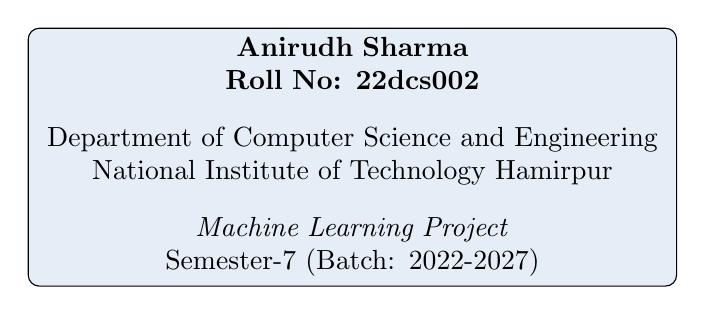
\begin{tikzpicture}
    \node[draw, fill=musicblue!10, rounded corners, text width=8cm, align=center] {
        \textbf{Anirudh Sharma} \\
        \textbf{Roll No: 22dcs002} \\
        \vspace{0.3cm}
        Department of Computer Science and Engineering \\
        National Institute of Technology Hamirpur \\
        \vspace{0.3cm}
        \textit{Machine Learning Project} \\
        Semester-7 (Batch: 2022-2027)
    };
\end{tikzpicture}

\vspace{0.2cm}
\textcolor{musicorange}{\rule{0.6\textwidth}{2pt}}

\vspace{0.2cm}
\textit{\small "Discovering musical patterns through unsupervised learning"}
\end{center}
\end{frame}

\end{document}
